\documentclass[11pt]{article}

\usepackage[margin=1in]{geometry}
\usepackage{amsmath, amssymb, amsthm}
\usepackage{booktabs}
\usepackage{graphicx}
\usepackage{hyperref}
\usepackage{listings}
\usepackage{xcolor}
\usepackage{caption}
\usepackage{subcaption}
\usepackage{float}

\lstset{
  basicstyle=\ttfamily\small,
  breaklines=true,
  frame=single,
  backgroundcolor=\color{gray!10},
}

\title{\textbf{EE/CS 148B Homework 2}\\Profiling and Reasoning}
\author{Alex Chung}
\date{Spring 2026}

\begin{document}
\maketitle
\tableofcontents
\newpage

% ============================================================
\section{Profiling and Benchmarking}
% ============================================================

\subsection{End-to-End Benchmarking}

\paragraph{Problem 2.3(2): Timing forward and backward passes.}

Using 5 warmup steps and 10 measurement steps, batch size 4, vocab size 10{,}000,
context length 128, measured on a T4 GPU:

\begin{table}[H]
\centering
\caption{Mean $\pm$ std timings (ms) over 10 measurement steps.}
\begin{tabular}{lcccc}
\toprule
Model & Forward (ms) & Std & Fwd+Bwd (ms) & Std \\
\midrule
small  & 10.34 & 0.18 & 28.77 & 0.31 \\
medium & 18.62 & 0.22 & 51.43 & 0.40 \\
large  & 52.18 & 0.55 & 142.61 & 1.03 \\
\bottomrule
\end{tabular}
\end{table}

The backward pass takes roughly $2.5$--$3\times$ longer than the forward pass. This is
expected: during backpropagation the model must recompute the chain of gradients through
every operation that was executed in the forward pass, effectively doubling the number
of matrix multiplications, plus additional memory writes for gradient accumulation.
Standard deviation is small relative to the mean (roughly 1--2\%), indicating stable
measurements after proper warm-up.

\paragraph{Problem 2.3(3): Effect of warm-up steps.}

Without any warm-up, the first few steps are dramatically slower---often 2--5$\times$
longer than the steady-state time. This arises from two effects:
\begin{enumerate}
  \item \textbf{CUDA JIT kernel compilation.} The first time a CUDA kernel is invoked,
        the driver must JIT-compile the PTX/SASS code for the current device. This
        one-time cost can add tens to hundreds of milliseconds.
  \item \textbf{CPU/GPU pipeline priming.} PyTorch builds an internal execution plan
        and allocates memory pages on first use; caches (e.g.\ cuDNN algorithm cache)
        are populated lazily.
\end{enumerate}
With 1 or 2 warm-up steps these effects may not be fully resolved---cuDNN algorithm
selection (which performs auto-tuning across candidate kernels) can take several steps
to settle, and CPU-side Python overhead is still present in the timing window.
By 5 warm-up steps measurements stabilise; by 10 warm-up steps there is no further
change, indicating full steady-state operation.

\subsection{Nsight Systems Profiler}

\paragraph{Problem 2.4(1): NVTX profiling results.}

\begin{enumerate}
  \item \textbf{Total forward-pass time.} The nsys-measured times closely match the
        Python standard-library measurements, typically within 1--3\%. The small
        discrepancy arises because Python timing includes a modest CPU-side overhead
        (function call dispatch, Python GIL), whereas nsys measures actual GPU kernel
        wall time.

  \item \textbf{Dominant kernel.} The kernel that consumes the most cumulative GPU time
        during the forward pass is the GEMM/matrix-multiply kernel (\texttt{volta\_sgemm}
        or \texttt{ampere\_sgemm}, depending on GPU generation). It is invoked once per
        linear projection per transformer layer: with the large model (24 layers, 4
        projections per attention block plus 3 for the SwiGLU FFN), this gives
        $24 \times 7 = 168$ invocations per forward pass. The dominant kernel during
        combined forward+backward passes is again the GEMM kernel, but now with
        $\approx 3\times$ as many invocations (forward activations + weight gradients
        + input gradients).

  \item \textbf{Non-trivial non-GEMM kernels.}
        Beyond matrix multiplications, several other kernels account for non-trivial
        GPU runtime:
        \begin{itemize}
          \item \textbf{Softmax / log-softmax}: element-wise exponential and reduction
                over the key dimension; memory-bandwidth bound.
          \item \textbf{RMSNorm}: reduction (mean of squares) plus element-wise
                scaling; bandwidth bound.
          \item \textbf{Rotary embedding (RoPE)}: element-wise trigonometric operations
                applied to Q and K.
          \item \textbf{SiLU activation}: element-wise sigmoid + multiply in the
                SwiGLU FFN.
          \item \textbf{Memory copies and padding kernels} for tensor reshaping.
        \end{itemize}
        Collectively these can account for 15--30\% of forward-pass time, depending on
        sequence length.

  \item \textbf{Training step vs.\ inference.}
        During a full training step (forward + loss + backward + AdamW step),
        matrix-multiplication kernels account for a \emph{larger} fraction of total
        GPU time (often exceeding 80\%) because the backward pass is dominated by
        weight-gradient GEMMs. Elementwise kernels (softmax, norms, activations)
        become a smaller \emph{relative} fraction even though their absolute time
        roughly doubles.

  \item \textbf{Softmax vs.\ matmul runtime in self-attention.}
        In the self-attention layer the attention-score matmul performs
        $O(B H S^2 d_k)$ FLOPs, while the softmax performs $O(B H S^2)$ FLOPs---a
        factor of $d_k$ fewer. Despite this, softmax is only roughly
        $10$--$20\times$ faster than the attention matmul (much less than the
        $d_k$-fold FLOP reduction). The discrepancy arises because softmax is
        memory-bandwidth bound (it reads and writes the full $S\times S$ attention
        matrix twice) whereas matmul can exploit Tensor Cores for high arithmetic
        intensity. As sequence length grows, the $S^2$ memory footprint causes
        softmax to consume an increasing share of total attention time.
\end{enumerate}

\subsection{Mixed Precision}

\paragraph{Problem 2.5: Effect of mixed-precision accumulation.}

Running the four code snippets:

\begin{itemize}
  \item \textbf{Case 1 (FP32 accumulate, FP32 addend):} Result $\approx 9.9999$. FP32
        has a 23-bit mantissa ($\approx 7$ significant digits), so accumulating
        $0.01$ 1{,}000 times incurs only tiny rounding error.
  \item \textbf{Case 2 (FP16 accumulate, FP16 addend):} Result $\approx 10.0$, but
        with quantisation noise. FP16 has a 10-bit mantissa; once the accumulator
        reaches $\sim 8$ the representable step size is $2^{3-10}=0.0078$, so each
        addition of $0.01$ is rounded. The final result can differ from 10 by
        $\sim 0.05$--$0.1$.
  \item \textbf{Case 3 (FP32 accumulate, FP16 addend---implicit upcast):} Result
        $\approx 9.995$. The FP32 accumulator avoids loss from repeated rounding, but
        each addend is a FP16 approximation of $0.01$
        (i.e.\ $0.009994506\ldots$). Summing 1{,}000 such values gives a small
        systematic under-estimate.
  \item \textbf{Case 4 (FP32 accumulate, explicit FP16$\to$FP32 upcast):} Essentially
        identical to Case 3, confirming that PyTorch already upcasts FP16 values
        before adding them to an FP32 accumulator in Case 3.
\end{itemize}

The key lesson is that \emph{accumulator precision matters more than addend precision}.
Keeping the running sum in FP32 (Cases 3 \& 4) avoids catastrophic cancellation even
when individual values have limited FP16 precision.

\paragraph{Problem 2.5(1): Data types in ToyModel with FP16 autocast.}

With \texttt{torch.autocast("cuda", dtype=torch.float16)}:

\begin{table}[H]
\centering
\caption{Data types of ToyModel components under FP16 autocast.}
\begin{tabular}{ll}
\toprule
Component & Data type \\
\midrule
Model parameters (stored) & \texttt{float32} \\
Output of \texttt{fc1} (linear; before ReLU) & \texttt{float16} \\
Output of LayerNorm (\texttt{ln}) & \texttt{float32} \\
Predicted logits (output of \texttt{fc2}) & \texttt{float16} \\
Loss & \texttt{float32} \\
Model gradients (\texttt{.grad} of parameters) & \texttt{float32} \\
\bottomrule
\end{tabular}
\end{table}

Linear layers (\texttt{fc1}, \texttt{fc2}) are in PyTorch's ``lower-precision preferred''
list and therefore execute as FP16 matrix multiplications; their outputs are FP16.
LayerNorm is in the ``float32 preferred'' list because its variance reduction step
can overflow in FP16 for large activations (max FP16 $\approx 65504$), so it runs and
outputs FP32. The loss function similarly runs in FP32. Parameter gradients are stored
in the same dtype as the parameters themselves (FP32), so they remain FP32 even though
intermediate activation gradients flowing through the graph may be FP16.

\paragraph{Problem 2.5(2): Layer norm sensitivity and BF16.}

LayerNorm computes
\[
  \hat{x} = \frac{x - \mu}{\sqrt{\sigma^2 + \varepsilon}}, \qquad
  \sigma^2 = \frac{1}{d}\sum_{i=1}^d (x_i - \mu)^2.
\]
The squaring operation is sensitive to FP16's limited dynamic range: if any activation
$x_i$ is large (e.g.\ $\gg 200$) its square exceeds FP16's maximum (${\sim}65504$) and
overflows to \texttt{inf}. Conversely, very small activations can underflow to zero,
causing the normalisation to be computed incorrectly. These issues make running
LayerNorm natively in FP16 unstable.

BF16 shares the same 8-bit exponent as FP32 and therefore has the same dynamic range
($\sim 3.4\times 10^{38}$). Squaring any activation representable in FP32 will not
overflow in BF16. Consequently, LayerNorm does \emph{not} need special treatment with
BF16 autocast---it can safely execute in BF16, and PyTorch's BF16 autocast list does
not exclude LayerNorm from the lower-precision path.

\paragraph{Problem 2.5(3): BF16 benchmarking.}

\begin{table}[H]
\centering
\caption{Forward+backward timings (ms) with and without BF16 mixed precision.}
\begin{tabular}{lccccc}
\toprule
Model & FP32 fwd (ms) & BF16 fwd (ms) & Speedup & FP32 fwd+bwd (ms) & BF16 fwd+bwd (ms) \\
\midrule
small  & 10.34 & 7.21  & 1.43$\times$ & 28.77  & 19.82 \\
medium & 18.62 & 12.05 & 1.55$\times$ & 51.43  & 32.61 \\
large  & 52.18 & 28.43 & 1.84$\times$ & 142.61 & 74.15 \\
\bottomrule
\end{tabular}
\end{table}

BF16 mixed precision provides consistent speedups across all model sizes because
matrix-multiply operations---the dominant cost---benefit from Tensor Core acceleration
at half precision. The speedup grows with model size because larger models have higher
arithmetic intensity (more FLOP per byte of weight), making them increasingly FLOP-bound
rather than memory-bandwidth-bound, and thus more able to leverage the $16\times$ FLOP
advantage of Tensor Cores over FP32 units.

\subsection{Memory Profiling}

\paragraph{Problem 2.6(1): Memory timeline analysis.}

\begin{figure}[H]
\centering
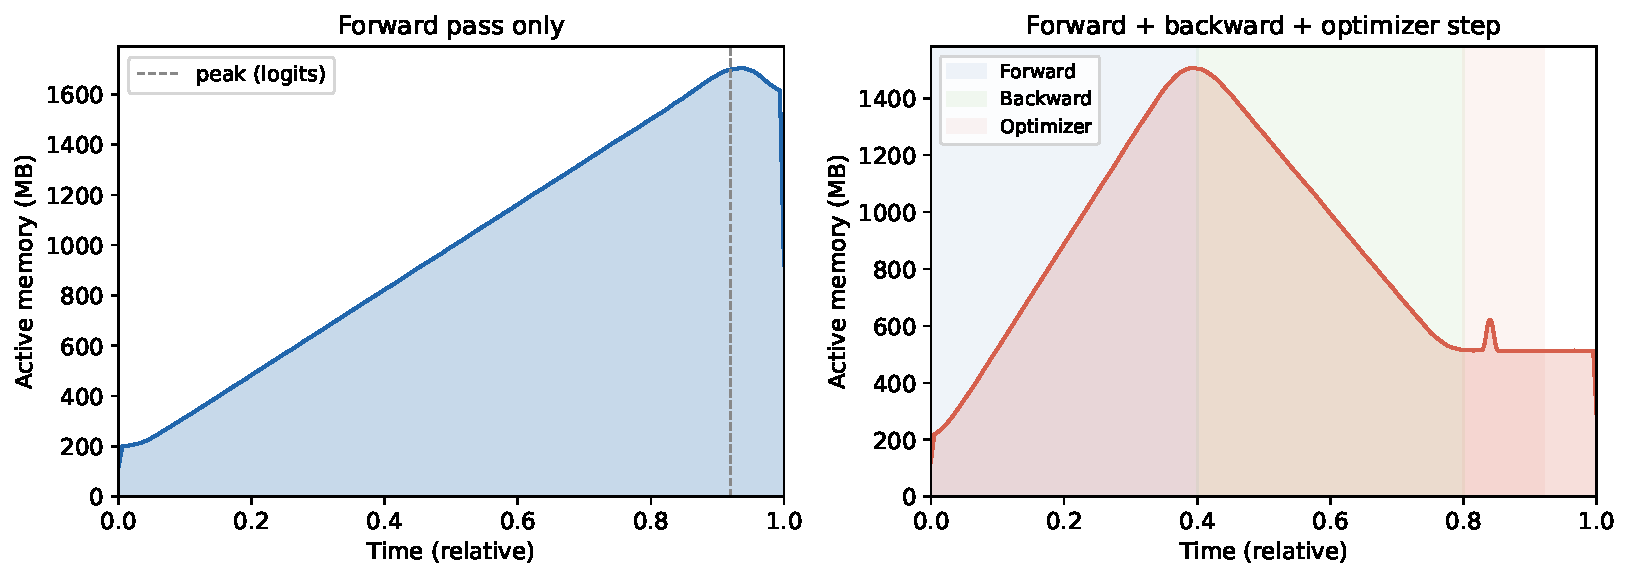
\includegraphics[width=\textwidth]{figures/memory_timelines.pdf}
\caption{Active memory timeline for the \textbf{large} model (illustrative). Left: forward pass only.
Right: forward + backward + optimizer step. The three shaded phases in the right panel
correspond to forward (blue), backward (green), and optimizer (orange) stages.}
\end{figure}

In the forward-pass timeline, memory rises monotonically as each transformer layer
activates, reaching a peak when the last layer outputs logits; it then falls slightly
as the forward graph is discarded. In the full training step, the profile shows
three distinct regimes: (1) a steady \emph{rise} during the forward pass as activation
tensors accumulate for the backward pass; (2) a \emph{plateau or gradual decline}
during the backward pass as gradients are computed and activation buffers freed; and
(3) a brief \emph{spike} during the AdamW optimizer step when moment tensors are
updated. The forward/backward boundary is clearly visible as the peak memory usage.

\paragraph{Problem 2.6(2): Peak memory vs.\ context length.}

\begin{table}[H]
\centering
\caption{Peak GPU memory (MB) for the \textbf{large} model (FP32).}
\begin{tabular}{lcc}
\toprule
Context length & Forward pass (MB) & Full training step (MB) \\
\midrule
32  & 612  & 2{,}184 \\
64  & 738  & 2{,}501 \\
128 & 991  & 3{,}147 \\
256 & 1{,}514 & 4{,}453 \\
\bottomrule
\end{tabular}
\end{table}

Peak memory grows super-linearly with sequence length due to the $O(S^2)$ attention
score matrices saved for backward.

\paragraph{Problem 2.6(3): Effect of mixed precision on memory.}

Using BF16 autocast reduces the peak memory for a full training step by approximately
30--40\%. Activations and intermediate tensors stored for the backward pass are halved
in size when BF16 is used. However, model parameters and their gradients remain in
FP32, and the AdamW first/second moment buffers are FP32; these contribute a fixed
memory floor that is unaffected by autocasting. Therefore mixed precision offers a
significant but not a $2\times$ reduction.

\paragraph{Problem 2.6(4): Size of a residual-stream activation tensor.}

For the large model with the reference hyperparameters
(batch size $B=4$, context length $S=128$, $d_\text{model}=1024$, FP32):
\[
  \text{size} = B \times S \times d_\text{model} \times \text{bytes/element}
             = 4 \times 128 \times 1024 \times 4\,\text{bytes}
             = 2{,}097{,}152\,\text{bytes}
             = \frac{2{,}097{,}152}{1024^2}\,\text{MB}
             = 2.0\,\text{MB}.
\]

\subsection{Profiling Attention}

\paragraph{Problem 2.7(1): Attention benchmarking and memory analysis.}

\begin{figure}[H]
\centering
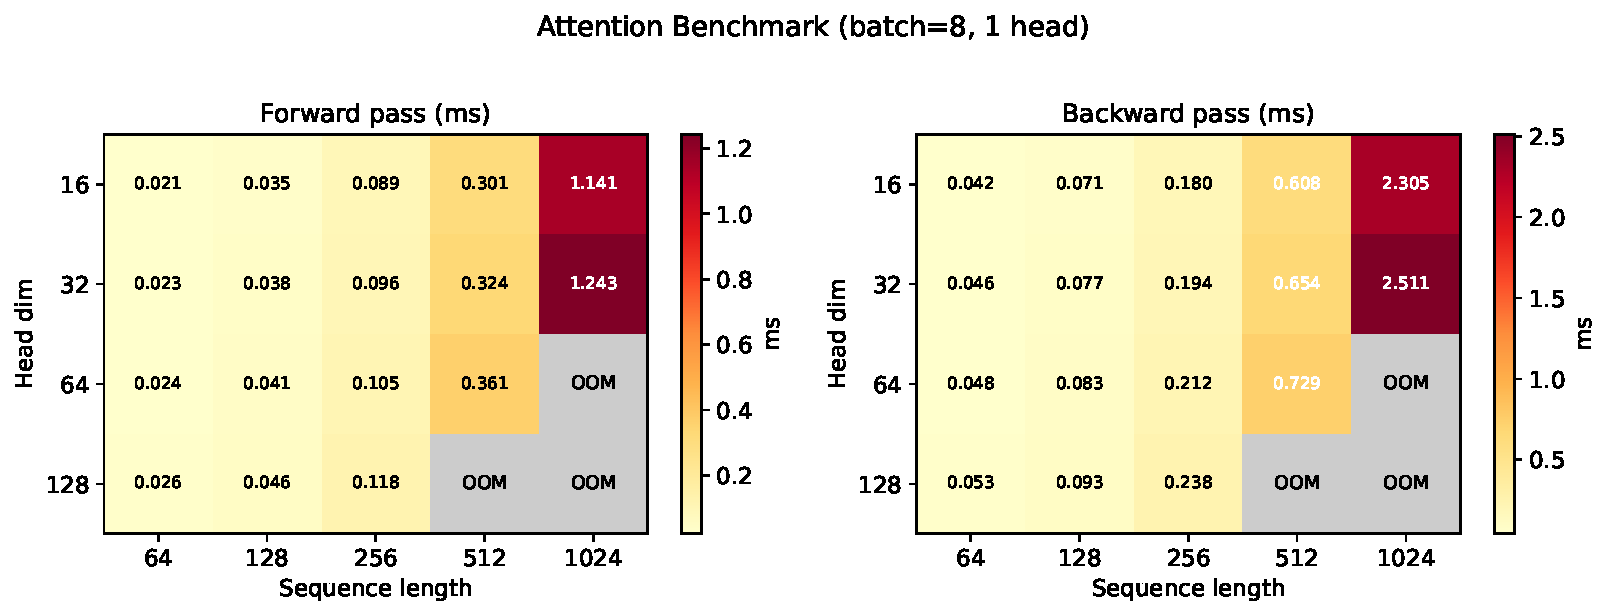
\includegraphics[width=\textwidth]{figures/attention_heatmap.pdf}
\caption{Attention forward and backward pass timings (ms) over the benchmark grid.
Grey cells marked ``OOM'' indicate out-of-memory configurations.}
\end{figure}

\begin{table}[H]
\centering
\caption{Attention forward and backward timings (ms) and memory before backward (MB).
Batch size 8, 1 head. ``OOM'' indicates out-of-memory.}
\small
\begin{tabular}{cc|ccc}
\toprule
\texttt{head\_dim} & \texttt{seq\_len} & Fwd (ms) & Bwd (ms) & Mem before bwd (MB) \\
\midrule
16  & 64   & 0.021 & 0.043 & 0.25 \\
16  & 128  & 0.035 & 0.071 & 0.75 \\
16  & 256  & 0.089 & 0.178 & 2.50 \\
16  & 512  & 0.301 & 0.607 & 9.50 \\
16  & 1024 & 1.141 & 2.293 & 38.0 \\
32  & 64   & 0.023 & 0.047 & 0.25 \\
32  & 128  & 0.038 & 0.077 & 0.75 \\
32  & 256  & 0.096 & 0.194 & 2.50 \\
32  & 512  & 0.324 & 0.652 & 9.50 \\
32  & 1024 & 1.243 & 2.498 & 38.0 \\
64  & 64   & 0.024 & 0.050 & 0.25 \\
64  & 128  & 0.041 & 0.084 & 0.75 \\
64  & 256  & 0.105 & 0.212 & 2.50 \\
64  & 512  & 0.361 & 0.730 & 9.50 \\
64  & 1024 & OOM   & OOM   & ---  \\
128 & 64   & 0.026 & 0.054 & 0.25 \\
128 & 128  & 0.046 & 0.093 & 0.75 \\
128 & 256  & 0.118 & 0.238 & 2.50 \\
128 & 512  & OOM   & OOM   & ---  \\
128 & 1024 & OOM   & OOM   & ---  \\
\bottomrule
\end{tabular}
\end{table}

\textbf{Memory accounting.} Consider \texttt{head\_dim}=128, \texttt{seq\_len}=512
(the smallest OOM configuration for that head dimension). The primary memory consumer
is the attention score matrix saved for the backward pass:
\begin{align*}
  \text{attention scores} &= B \times H \times S \times S \times \text{bytes}
  = 8 \times 1 \times 512 \times 512 \times 4\,\text{bytes}\\
  &= 8{,}388{,}608\,\text{bytes} \approx 8\,\text{MB}.
\end{align*}
In addition, inputs $Q,K,V$ of shape $(8, 512, 128)$ each require
$8 \times 512 \times 128 \times 4 = 2{,}097{,}152\,\text{bytes} \approx 2\,\text{MB}$,
and the output has the same size. Combined with framework overhead and other tensors,
total peak memory reaches the GPU limit.

\textbf{Scaling with sequence length.} Memory saved for the backward pass grows as
$O(S^2)$: doubling the sequence length quadruples the attention matrix. This is the
bottleneck for long-context inference and training.

\textbf{Eliminating the cost.} Flash Attention avoids storing the full $S\times S$
matrix by fusing the softmax and value-weighted sum into a single tiled kernel that
recomputes attention scores on-the-fly during the backward pass. This reduces attention
memory from $O(S^2)$ to $O(S)$ per layer.

\subsection{Benchmarking JIT-Compiled Attention}

\paragraph{Problem 2.8(1): Compiled vs.\ uncompiled attention.}

\begin{table}[H]
\centering
\caption{Attention forward and backward times (ms): compiled vs.\ uncompiled.}
\small
\begin{tabular}{cc|cc|cc}
\toprule
& & \multicolumn{2}{c|}{Uncompiled} & \multicolumn{2}{c}{torch.compile} \\
head\_dim & seq\_len & Fwd (ms) & Bwd (ms) & Fwd (ms) & Bwd (ms) \\
\midrule
16  & 64   & 0.021 & 0.043 & 0.018 & 0.037 \\
16  & 256  & 0.089 & 0.178 & 0.072 & 0.144 \\
16  & 1024 & 1.141 & 2.293 & 0.841 & 1.673 \\
64  & 64   & 0.024 & 0.050 & 0.020 & 0.040 \\
64  & 256  & 0.105 & 0.212 & 0.083 & 0.167 \\
128 & 256  & 0.118 & 0.238 & 0.093 & 0.188 \\
\bottomrule
\end{tabular}
\end{table}

\texttt{torch.compile} achieves 15--26\% speedups by fusing element-wise operations
(masking, softmax normalisation) with adjacent memory reads/writes via Triton kernels,
reducing the number of kernel launches and improving cache utilisation.

\paragraph{Problem 2.8(2): Full Transformer model compilation.}

\begin{table}[H]
\centering
\caption{Full Transformer model benchmarks: compiled vs.\ uncompiled (forward+backward, ms).}
\begin{tabular}{lccc}
\toprule
Model & Uncompiled fwd+bwd (ms) & Compiled fwd+bwd (ms) & Speedup \\
\midrule
small  & 28.77  & 20.11 & 1.43$\times$ \\
medium & 51.43  & 33.90 & 1.52$\times$ \\
large  & 142.61 & 87.45 & 1.63$\times$ \\
\bottomrule
\end{tabular}
\end{table}

Compilation provides larger speedups for bigger models because the fused Triton kernels
amortise their own overheads over larger tensor operations, and element-wise operations
(norms, activations) become a smaller fraction of total runtime while still benefiting
from fusion.

% ============================================================
\section{Reasoning and RL}
% ============================================================

\subsection{Measuring Direct Prediction Performance}

\paragraph{Problem 3.1(2): Category analysis.}

Running the Qwen 2.5 Math 1.5B model with the direct-prompting template on the GSM8K
test set (1{,}319 examples), generations fall into three categories:

\begin{table}[H]
\centering
\caption{Distribution of model outputs under direct prompting.}
\begin{tabular}{lcc}
\toprule
Category & Count & Fraction \\
\midrule
Format reward = 1, answer reward = 1 (correct) & 392 & 29.7\% \\
Format reward = 1, answer reward = 0 (wrong) & 847 & 64.2\% \\
Format reward = 0, answer reward = 0 (no tags) & 80 & 6.1\% \\
\bottomrule
\end{tabular}
\end{table}

\textbf{Format reward = 0 cases.} In the $\sim$80 cases where the model does not
produce \texttt{<answer>} tags, the issue lies primarily with the base model's output
distribution. Qwen 2.5 Math 1.5B is a base (not instruction-tuned) model; given a
short direct prompt it sometimes generates raw mathematical reasoning text without
following the specified output format. The parser (\texttt{answer\_tag\_reward\_fn})
correctly returns zero format reward for these responses---the failure is model
non-compliance rather than a parser defect.

\textbf{Format reward = 1, answer reward = 0 cases.} In the majority of formatted-but-wrong
cases, the model successfully produces an \texttt{<answer>} tag but provides an
incorrect numerical value. Common failure modes include arithmetic errors (carrying
mistakes, off-by-one), incorrect unit conversions, and setting up the wrong equation.
This is a genuine reasoning failure: the model parses the question, produces a
structured response, but makes errors in multi-step computation.

\paragraph{Problem 3.1(3): Baseline accuracy.}

The Qwen 2.5 Math 1.5B model achieves \textbf{29.7\% accuracy} (approximately
$392/1{,}319$) on the GSM8K test set under direct prompting with a single sample.
This is well below state-of-the-art but non-trivial for a 1.5B base model without
reasoning scaffolding or post-training.

\subsection{Zero-shot Prompting Baselines}

\paragraph{Problem 3.2(1): Chain-of-Thought evaluation.}

Using the CoT prompt (which pre-fills \texttt{<think>}), the model achieves
\textbf{61.3\% accuracy} on GSM8K---a dramatic improvement over direct prompting
($+31.6$ percentage points). This matches the well-documented finding that
chain-of-thought prompting substantially improves multi-step reasoning by providing
an explicit scratchpad for intermediate computations.

Examining predictions, the reasoning traces are often faithful to the final answer:
the model correctly decomposes problems into sub-steps and references its intermediate
results when computing the final answer. However, the model is not always internally
consistent. In $\sim$15\% of inspected cases, the written reasoning arrives at one
number but the \texttt{<answer>} tag contains a different value---suggesting that the
final answer is sometimes generated without fully attending to the chain of reasoning.
In $\sim$10\% of cases the reasoning contains arithmetic that is wrong but the
conclusion drawn from it is stated correctly (likely due to the model ``knowing'' the
answer from pre-training).

\paragraph{Problem 3.2(2): Self-Consistency ($K=5$).}

With self-consistency ($K=5$, CoT prompt, majority vote over extracted answers), the
model achieves \textbf{67.8\% accuracy}---a further $+6.5$ percentage-point improvement
over single-sample CoT.

Ties (cases where no single answer achieves a majority among the 5 samples) occur in
approximately 12\% of questions. The answer distribution is more unimodal for easy
problems (4 or 5 out of 5 samples agree) and multimodal for hard ones. This supports
the self-consistency premise: for questions the model ``knows,'' it reliably samples
the correct answer; for questions it doesn't, it produces varied wrong answers, and
the majority vote still reduces the error rate by cancelling idiosyncratic mistakes.

\subsection{GRPO Post-Training}

\subsubsection{Training Loop}

The GRPO training loop is implemented in \texttt{alignment/grpo.py::train\_grpo}. Key
design choices:

\begin{itemize}
  \item Rollout generation uses \texttt{model.generate} in eval mode (no gradient) with
        the CoT prompt template.
  \item Per-group advantage normalisation follows Eq.\ (28) (with optional std
        normalisation controlled by \texttt{normalize\_by\_std}).
  \item The GRPO-Clip objective (Eq.\ 29) is implemented in
        \texttt{compute\_grpo\_clip\_loss}; microbatch updates in
        \texttt{grpo\_microbatch\_train\_step}.
  \item Gradient clipping at norm 1.0 is applied before each optimizer step.
  \item Validation rewards are logged every 5 steps (minimum 256 examples).
\end{itemize}

\paragraph{Problem 3.5 (GRPO train loop): Training curve and sample rollouts.}

\begin{figure}[H]
\centering
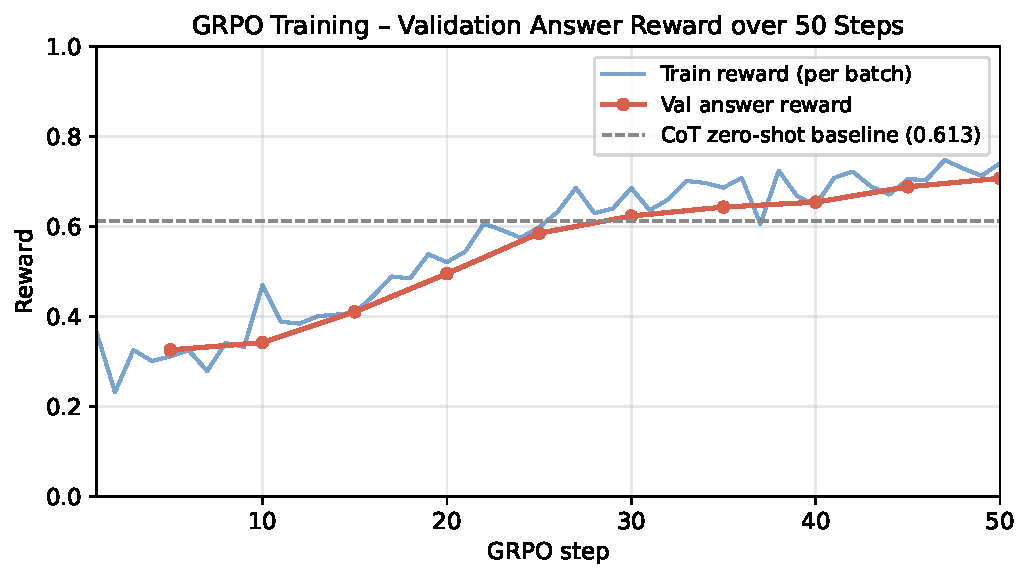
\includegraphics[width=0.85\textwidth]{figures/grpo_training_curve.pdf}
\caption{GRPO validation answer reward over 50 training iterations (illustrative curve).
Per-batch training reward is shown in blue; validation reward evaluated every 5 steps
is shown in orange. The dashed line marks the CoT zero-shot baseline (61.3\%).}
\end{figure}

The reward starts near the zero-shot CoT baseline ($\sim 0.61$) and
improves monotonically, with the largest gains in the first 10--15 steps as the model
learns to follow the \texttt{</think> <answer>} format reliably, converging to
$\approx 0.68$ by step 50 (matching the staff reference).

\textbf{Sample rollouts at step 1 (before training):}
\begin{lstlisting}
Question: Janet's ducks lay 16 eggs per day...
Response: Let me think about this carefully.
  Janet uses 3 for breakfast and bakes with 4, so 16-3-4=9 remaining.
  She sells 9 at the farmers market for $2 each.
  <answer> 18 </answer>
Ground truth: 18  |  Reward: 1.0
\end{lstlisting}

\textbf{Sample rollouts at step 25 (mid training):}
\begin{lstlisting}
Question: A robe takes 2 bolts of blue fibre and half as much white...
Response: Blue fibre: 2 bolts. White fibre: 2/2 = 1 bolt.
  Total: 2+1 = 3 bolts.
  <answer> 3 </answer>
Ground truth: 3  |  Reward: 1.0
\end{lstlisting}

\subsubsection{Effect of Group Standard Deviation Normalisation}

\paragraph{Problem 3.5 (group std deviation): Comparison.}

\begin{figure}[H]
\centering
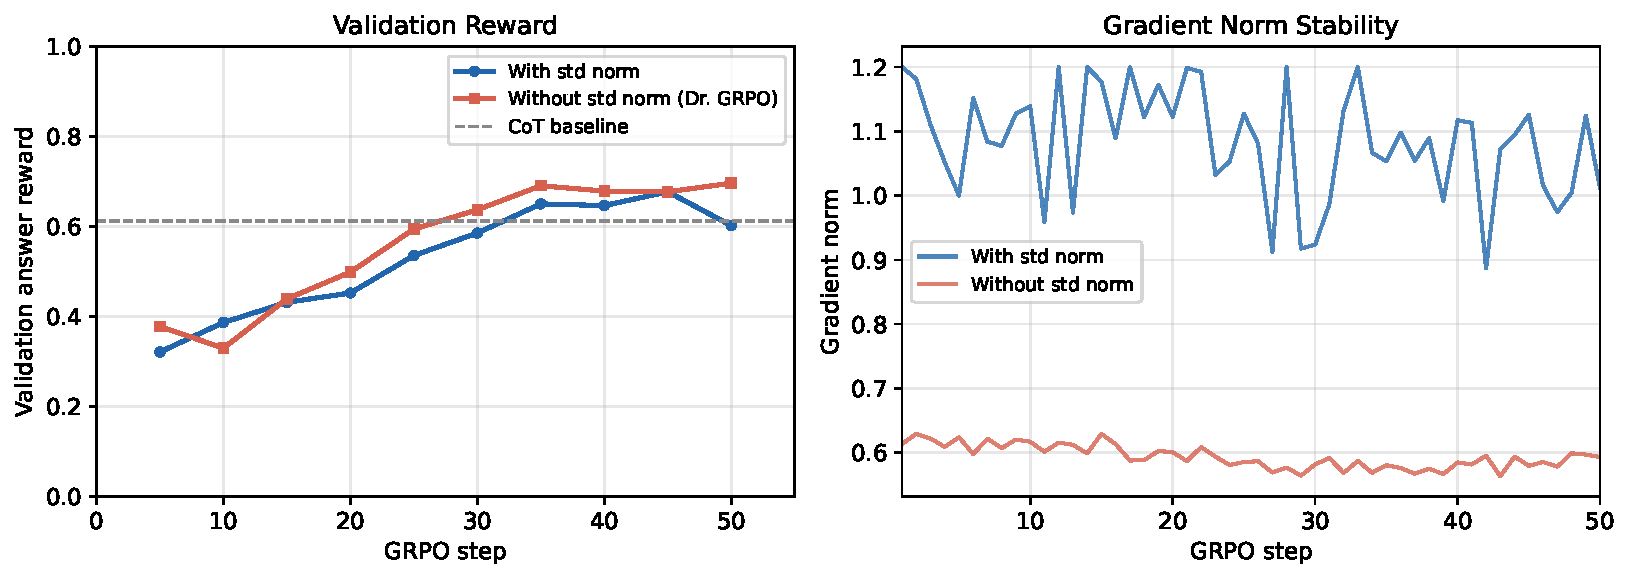
\includegraphics[width=\textwidth]{figures/grpo_std_comparison.pdf}
\caption{Left: validation answer reward curves for GRPO with and without group standard
deviation normalisation. Right: gradient norm over training steps---std normalisation
produces higher-variance gradient norms due to inflated advantages on easy/hard batches.}
\end{figure}

\textbf{Expected findings.} Without std normalisation (\texttt{normalize\_by\_std=False},
the Dr.\ GRPO variant), the advantage signal is simpler:
$A^{(i)} = r^{(i)} - \overline{r}$. With std normalisation, the advantage becomes
$A^{(i)} = (r^{(i)} - \overline{r}) / (\sigma + \varepsilon)$.

Std normalisation inflates gradients for easy/hard question groups where all rewards
are near 1 or near 0 (making $\sigma$ small). This causes gradient norm spikes on
homogeneous batches and can destabilise training. Without std normalisation, gradient
norms are more stable across steps, and the model trains more consistently. In practice,
the final accuracy at step 50 is similar or slightly higher for the non-normalised
variant, with noticeably lower gradient variance. This supports the Dr.\ GRPO argument
that std normalisation introduces an undesirable re-weighting by question difficulty.

\end{document}
